\documentclass[sigconf,anonymous]{acmart}

\usepackage{booktabs}
\usepackage{amsmath}
\usepackage{tikz}
\usetikzlibrary{arrows.meta,positioning,fit,backgrounds}
\usepackage{placeins}
\usepackage{algorithm}
\usepackage{algpseudocode}
\usepackage{cleveref}

\definecolor{tbdred}{RGB}{153,0,0}
\setlength{\emergencystretch}{3em}
\newcommand{\tbd}[1]{\textcolor{tbdred}{\texttt{#1}}}
\newcommand{\stg}{semantic trajectory graph}
\newcommand{\aeu}{Action execution unit}
\newcommand{\csg}{candidate subgraph}
\newcommand{\csmil}{contextual semantic-subgraph MIL}
\newcommand{\sexp}{safety experience}

\begin{document}

\title{Detect, Localize, and Defend: Action-Centered Semantic Trajectory Graphs for the Agentic Web}

\author{Anonymous Author(s)}
\affiliation{\institution{Anonymous Institution}\city{}\country{}}

\begin{abstract}
Language-model agents increasingly act on the Web through tools---searching, browsing, filling forms, and transacting on behalf of users---and every tool call can change external state. Existing screening either classifies flat text or scores an entire execution, leaving two questions unanswered: whether cross-step execution dependencies are represented at all, and which tool operation actually produced the risk. We reformulate agent risk analysis as joint graph-level anomaly detection and action-level subgraph localization over a \stg{} that encodes tasks, reasoning, tool calls, and environment states with typed, directed, and justified edges. We further propose \aeu{}s---inseparable semantic slices of intent, inputs, execution, and outcome---as the atomic unit of unit-wise \csg{}s, a \csmil{} model that aligns full trajectories and candidates through a shared edge-attention encoder and ranks risky actions under graph-level supervision with paired weak supervision, and \sexp{}s compiled from the top-ranked Action subgraph that condition later agent decisions, closing the loop from detection to defense; across \tbd{TBD-EVALUATION-SCOPE}, the proposed method achieves \tbd{TBD-KEY-RESULTS} under \tbd{TBD-PROTOCOL}.
\keywords{agentic web, LLM agents, graph anomaly detection, subgraph localization, safety experience}
\ccsdesc[500]{Security and privacy~$\rightarrow$~Intrusion detection systems}
\ccsdesc[300]{Computing methodologies~$\rightarrow$~Artificial intelligence}
\end{abstract}

\maketitle

\section{Introduction}

The Web is entering a phase in which a growing share of interactions is performed by software on behalf of people. Language-model agents interleave natural-language reasoning with tool calls to search, browse, fill forms, send messages, and transact~\cite{yao2022react,schick2023toolformer}, and standardized tool interfaces such as the Model Context Protocol turn external services and data sources into first-class agent capabilities~\cite{hou2025model,zhang2025security}. Web-native benchmarks demonstrate agents operating realistic sites end to end~\cite{zhou2023webarena,deng2023mindweb}, tool-use suites exercise stateful, multi-step interactions~\cite{liu2023agentbench,lu2024toolsandbox}, API-based agents extend the reach of browsing~\cite{song2024beyond}, agentic search systems now return synthesized, citation-backed answers instead of link lists~\cite{gou2025mindweb}, and survey literature describes the resulting environment as an \emph{agentic Web} in which autonomous, goal-driven agents are primary actors~\cite{yang2025agentic,nie2026synergy,zhang2024large}. This shift reopens long-standing assumptions about who reads, writes, and pays for the Web, because the client is no longer a human reading a page but an agent executing operations---and every executed tool call can change external state.

The same shift changes the attack surface. Under indirect prompt injection, hostile instructions embedded in fetched content steer the model that processes them~\cite{greshake2023what,liu2023prompt,liu2024automatic}; when the steered model is an agent, the instruction is executed through tools with real consequences~\cite{zhan2024injecagent,debenedetti2024agentdojo,zhang2024agent}. Attacks and evaluations have followed this trajectory: environmental injection on generalist web agents~\cite{liao2024environmental}, prompt injection against multimodal web agents~\cite{wang2025webinject}, tool-layer attacks on protocol-mediated tool use~\cite{wang2026adaptools}, adaptive red-teaming of deployed web agents~\cite{syros2026muzzle}, and analyses showing that web agents are more vulnerable than standalone models precisely because each step multiplies exposure~\cite{chiang2025agents}. Attack success is commonly measured as an attack success rate over task runs~\cite{debenedetti2024agentdojo,zhan2024injecagent}, and dedicated safety benchmarks confirm that autonomous web agents routinely complete tasks in policy-violating ways~\cite{tur2025safearena,levy2024stwebagentbench}. Crucially for the Web, consequences are state changes---payments sent, records modified, private data exfiltrated---and recent work shows such consequences can be made covert, so the user never learns what their agent did~\cite{lee2026will}.

Current defenses address this threat at the wrong granularity, and their collective blind spots can be stated as two unanswered questions: whether cross-step execution dependencies are represented at all, and which tool operation actually produced the risk. The first question exposes segment-level methods. Content-level hardening and detection operate on text spans or attention patterns~\cite{chen2024struq,chen2024secalign,zhong2025attention}, guard models classify messages against safety taxonomies~\cite{inan2023llama,liu2024calibration}, and design-level systems constrain information flow between channels~\cite{debenedetti2025defeating,zhu2025melon}; all of them judge \emph{segments} in isolation, while the risk of an agent run is a property of \emph{compositions}: a benign query, a benign-looking tool output, and an otherwise reasonable plan can jointly produce an unauthorized transfer, and no per-segment verdict sees that propagation. The second question exposes run-level methods. Whole-trajectory judges score an entire execution~\cite{yuan2024rjudge,zhuge2024agentasajudge,mohammadi2026trajectoryjudge} and runtime monitors predict or veto upcoming steps~\cite{luo2025agrail,wang2025probguard,lin2026dreamguard,mou2026toolsafe,liu2026agentdog}; they answer \emph{whether} a run went bad, but not \emph{which} operation caused it, and outcome-only judges demonstrably miss process faults that do not change the final result~\cite{mohammadi2026trajectoryjudge}. An alert without a locus cannot become policy for the agent, cannot be audited by a site operator, and cannot be accumulated as knowledge; and since guardrails themselves are attackable and their verdicts are sensitive to formulation~\cite{zhou2026from}, evidence that is checkable and reusable has independent value.

We argue that the root cause of both gaps is a mismatch between the unit of risk and the unit of execution. Risk in tool-using agents propagates along real execution dependencies: external state enters through a tool result, is adopted by reasoning, and materializes in a tool call whose output becomes the next context. The natural boundary of this propagation is the \emph{action}: one tool call together with the state it consumed, the reasoning that justified it, and the state it produced. Reasoning has long been modeled as graphs in prompting frameworks~\cite{yao2023tree,besta2023graph}, and recent failure-attribution work shows that decisive errors can lie many steps away from their visible consequences, making dependency structure essential for locating them~\cite{deng2026defa}. Yet no existing representation binds risk evidence to complete tool operations: fixed-$k$-hop neighborhoods cut through operations at arbitrary points, keeping half of a reasoning chain while discarding the state that motivated it.

This paper makes the \aeu{} the anchor of agent safety analysis. We represent each execution as a directed \stg{} whose nodes are problems, thoughts, actions, and states, and whose typed and directed edges carry justification text. We construct, for every action, an inseparable \aeu{} and expand \csg{}s by adding whole predecessor units along real dependencies, so that every candidate is a complete, connected slice of an actual execution. A \csmil{} model encodes the full trajectory and all candidates with a shared edge-attention encoder, fuses local scores with the global score, and is trained with graph-level labels plus paired weak supervision derived from normal/anomalous executions of the same task, whose changed actions identify likely loci. At inference, a validated threshold triggers candidate ranking, and the top-ranked Action subgraph is compiled by a generator---which never sees ground-truth labels---into a structured \sexp{} that conditions the agent's subsequent decisions, closing the loop from detection to defense. Our contributions are:
\begin{itemize}
  \item a directed \stg{} representation for tool-using agents that jointly encodes tasks, reasoning, tool calls, and environment states, with the semantic type, direction, and justification of every edge;
  \item a \csg{} extraction and graph-level anomaly detection scheme in which \csg{}s are built on \aeu{}s---complete tool operations rather than fixed-hop neighborhoods---and a \csmil{} model that aligns full trajectories and candidates through a shared edge-attention encoder and, via learnable local--global aggregation and paired weak supervision, performs graph-level detection and Action-level localization jointly;
  \item a subgraph-level \sexp{} mechanism that compiles the top-ranked Action subgraph into a structured, node-grounded experience---generated without access to ground-truth labels---which conditions later agent decisions and closes the loop from detection to defense;
  \item an experimental design spanning detection, Action-level localization, and a controlled defense study whose conditions separate the effect of localized evidence from generic warning effects.
\end{itemize}
Section~\ref{sec:vision} develops why this formulation matters for the future Web: trajectory graphs as an auditable substrate and \sexp{}s as a portable safety layer. The rest of the paper formalizes the problem (\S\ref{sec:problem}), describes data and graph construction (\S\ref{sec:data}), details the method (\S\ref{sec:method}), specifies the evaluation design (\S\ref{sec:experiments}--\ref{sec:defense}), discusses implications for the agentic Web (\S\ref{sec:vision}), and concludes.

\section{Related Work}

\subsection{Attacks on Tool-Using and Web Agents}
Research on language-model security began with adversarial inputs to a single model but has moved decisively toward tool-mediated, multi-step settings. Indirect prompt injection showed that content fetched by an application can steer the model that reads it~\cite{greshake2023what,liu2023prompt}, and automated search over injection payloads generalizes the attack~\cite{liu2024automatic}. When the application is an agent, the injected instruction becomes executable: InjecAgent measures direct and indirect injections against tool-integrated agents~\cite{zhan2024injecagent}, AgentDojo provides a dynamic environment with adaptive attackers~\cite{debenedetti2024agentdojo}, and the Agent Security Bench formalizes attack scenarios across agent scenarios~\cite{zhang2024agent}. Web-specific work shows that hostile page content can hijack browsing agents to leak private data~\cite{liao2024environmental} or manipulate multimodal action generation~\cite{wang2025webinject}; protocol-level studies extend the surface to tool discovery and selection under MCP~\cite{hou2025model,zhang2025security,wang2026adaptools}; and red-teaming frameworks adaptively search web agents for injection chains~\cite{syros2026muzzle}. Security analyses attribute the elevated risk of web agents to multi-step processing of untrusted content~\cite{chiang2025agents}, and safety benchmarks for autonomous web agents document policy-violating completions~\cite{tur2025safearena,levy2024stwebagentbench}. Recent measurements emphasize a property directly relevant to detection: attacks can be made \emph{covert}, leaving no user-visible trace of the compromised operation~\cite{lee2026will}. Our work takes this multi-step, state-changing threat model as given and asks what representation makes the resulting risk detectable and attributable.

\subsection{Defenses: Content Hardening, Guards, Judges, and Runtime Monitors}
Defenses cluster by the object they inspect. Content-level methods restructure queries or align preferences so instructions hidden in data are not followed~\cite{chen2024struq,chen2024secalign}; attention-based detectors localize anomalous attention mass over injected spans~\cite{zhong2025attention}; provable and design-level approaches enforce data-flow and capability constraints that make injections inert~\cite{zhu2025melon,debenedetti2025defeating}. Guard models classify inputs and outputs against safety taxonomies~\cite{inan2023llama}, with known calibration limitations~\cite{liu2024calibration}. Judge-style assessment scores whole interactions or trajectories~\cite{zheng2023judging,yuan2024rjudge,zhuge2024agentasajudge}, and analysis of outcome-only trajectory judges shows they miss faults that do not alter the final result, arguing for process-level evidence~\cite{mohammadi2026trajectoryjudge}. Runtime monitors predict risky next actions or reason over world models~\cite{wang2025probguard,lin2026dreamguard}, adapt lifelong~\cite{luo2025agrail}, operate at step level~\cite{mou2026toolsafe}, or produce diagnostic explanations~\cite{liu2026agentdog}; guardrails themselves, however, can become denial-of-service targets and their verdicts are formulation-sensitive~\cite{zhou2026from}. Across these families, outputs are either a scalar over text or a verdict over a run; the operation-level evidence needed to reconfigure an agent is rarely produced, and when it is (as in diagnostic frameworks) it is not coupled to a learned detector that can rank \emph{which} operations are suspect. That coupling---joint detection, localization, and conversion into agent-consumable knowledge---is the gap this paper addresses.

\subsection{Graph Structure, Graph Anomaly Detection, and MIL}
Modeling reasoning as a graph has precedent in prompting frameworks that branch and merge thoughts~\cite{yao2023tree,besta2023graph}, and dependency-guided attribution over execution graphs recently showed that decisive failures must be located with structural context~\cite{deng2026defa}. On the modeling side, we build on attention-based and relational graph encoders~\cite{velikovi2017graph,brody2021attentive,schlichtkrull2017modeling,hu2020heterogeneous}. Graph anomaly detection offers detectors at node and graph levels~\cite{tang2022rethinking,liu2021anomaly,roy2024gadnr,duan2022arise}, including substructure-aware~\cite{duan2022arise} and subgraph-aligned formulations~\cite{hu2025samcl}, anomaly detection over edge-attributed multigraphs~\cite{sotiropoulos2023adamm}, and transferable graph-level scoring~\cite{wang2026glass}. These methods, however, target social, transaction, or sensor graphs whose anomalies are unusual nodes or subgraph motifs; none instantiates a graph over agent executions, where the anomaly of interest is a \emph{semantic} dependency pattern---an operation and its justification chain---rather than a structural outlier, and none provides operation-anchored localization. Multiple instance learning supplies the weak-supervision discipline we need: bag-level labels with instance-level ambiguity~\cite{carbonneau2016multiple}, attention-based aggregation~\cite{ilse2018attentionbased}, and graph-based bag encoders~\cite{tu2019multiple}. We instantiate bags as trajectories, instances as \aeu{}-anchored \csg{}s, and add paired supervision that classical MIL does not use.

\subsection{Experience, Reflection, and the Closest Work}
Agents already convert experience into reusable knowledge: verbal self-reflection improves retries~\cite{shinn2023reflexion}, experience-driven learners extract and transfer insights across tasks~\cite{zhao2023expel}, and recent systems industrialize reflective learning~\cite{allard2026experiential}; a unified review describes this trend as \emph{externalization} of memory, skills, and protocols around the model~\cite{zhou2026externalization}. This literature reuses experience for \emph{competence}; we reuse it for \emph{safety}, grounding each experience in a localized risk subgraph rather than a free-text lesson. The closest work to ours is DeFA~\cite{deng2026defa}, which attributes failures to decisive errors using dependency guidance over agent traces; DeFA is post-hoc---it explains failures after they are known---whereas our formulation detects anomalous trajectories \emph{before} outcomes are trusted, localizes risk at the granularity of complete tool operations under only graph-level supervision, and additionally converts the localized evidence into \sexp{}s that condition future behavior. Runtime governance proposals argue for contracts and policies at execution time~\cite{ng2026agent,joshi2026deontic,errico2025securing}; our detector and experience format are designed as the concrete substrate such contracts would audit.

\section{Problem Formulation}
\label{sec:problem}

\subsection{Tool-Using Agent Trajectories and Labels}
A \emph{trajectory} $\mathcal{T}$ records an agent run from receiving a task to producing a final result. It contains the user goal, plans and reflections, every tool invocation with its parameters, every environment-returned state, and the final result; implementations may interleave these records, and our representation only requires that each record carry its segment text and role. Each trajectory carries a graph label
\begin{equation}
y_G \in \{0,1\},
\label{eq:label}
\end{equation}
where $y_G=0$ denotes a normal completion or a successful defense against an attempted attack, and $y_G=1$ denotes that an attack produced a wrong, unauthorized, or leaking outcome. Data sources, labeling protocol, and quality control are reported as \tbd{TBD-DATA-PROVENANCE}, \tbd{TBD-LABELING-PROTOCOL}, and \tbd{TBD-DATA-QUALITY-CONTROL}.

\subsection{Semantic Trajectory Graph}
We represent $\mathcal{T}$ as a directed attributed graph
\begin{equation}
G=(V,E,X_V,X_E),
\label{eq:graph}
\end{equation}
where $V$ is the node set, $E\subseteq V\times V$ the directed edge set, and $X_V$, $X_E$ the node and edge features described in \S\ref{sec:data}. Nodes carry one of four types reflecting execution roles (Table~\ref{tab:nodetypes}), and edges carry one of five relation types reflecting execution semantics (Table~\ref{tab:edgetypes}).

\begin{table}[t]
\caption{Node types of the \stg{}.}
\label{tab:nodetypes}
\begin{tabular}{@{}lp{0.66\linewidth}@{}}
\toprule
Node type & Meaning \\
\midrule
\texttt{Problem} & user task or original goal \\
\texttt{Thinking} & agent plan, analysis, or reflection \\
\texttt{Action} & agent-initiated tool call \\
\texttt{State} & tool output, environment feedback, or final state \\
\bottomrule
\end{tabular}
\end{table}

\begin{table}[t]
\caption{Edge types of the \stg{}. Direction always follows execution flow.}
\label{tab:edgetypes}
\begin{tabular}{@{}lp{0.66\linewidth}@{}}
\toprule
Edge type & Meaning \\
\midrule
\texttt{computes\_from} & an Action produces a State \\
\texttt{depends\_on} & later reasoning or operation uses earlier information \\
\texttt{sequential} & execution-order relation only \\
\texttt{reflects} & reasoning or conclusion reflects a state \\
\texttt{branches\_from} & a plan branches from shared prior information \\
\bottomrule
\end{tabular}
\end{table}

\subsection{Action Execution Units}
For an action $a\in V$, the \aeu{} is the inseparable semantic slice
\begin{equation}
U_a=\{a\}\cup R_a\cup I_a\cup O_a\cup F_a,
\label{eq:unit}
\end{equation}
where $R_a$ is the \texttt{Thinking} chain recovered along semantic in-edges that justified $a$; $I_a$ is the set of \texttt{State}/\texttt{Problem} nodes feeding $a$ or its reasoning; $O_a$ is the \texttt{State} produced by $a$; and $F_a$ is the set of reflections or results directly tied to $O_a$. The typical structure is
\begin{center}
\emph{input State/Problem $\rightarrow$ Thinking chain $\rightarrow$ Action $\rightarrow$ output State,}
\end{center}
and the definition takes one complete tool operation as the minimal granularity rather than a node distance. This choice is deliberate: every candidate evaluated downstream corresponds to something the agent actually did, with the evidence that justified it attached.

\subsection{Dependency-Aware Candidates}
If the output state of unit $U_{a_i}$ is consumed by unit $U_{a_j}$, we add a unit dependency $U_{a_i}\rightarrow U_{a_j}$. For an anchor unit, candidates are grown by adding complete predecessor units layer by layer:
\begin{equation}
C_a^{(0)}=U_a,
\label{eq:cand0}
\end{equation}
\begin{equation}
C_a^{(l+1)}=C_a^{(l)}\cup\bigcup_{U_p\in\operatorname{Pred}(C_a^{(l)})}U_p .
\label{eq:cand}
\end{equation}
Candidates satisfy six constraints: each candidate is anchored at a real Action; all nodes and edges come from the original graph; each candidate is connected through real edges; each expansion adds complete execution units; independent branches form separate candidates while converging actions may form joint-context candidates; and the candidate budget may not remove every anchor candidate of any action. The candidate set of a trajectory is $\mathcal{C}=\{C_k\}$.

\subsection{Tasks}
Given $G$ with features and the candidate set $\mathcal{C}$, the model must solve three coupled tasks. \emph{Graph-level detection}: estimate $p_G=\Pr(y_G=1\mid G)$. \emph{Action-level localization}: rank candidates $C_k\in\mathcal{C}$ by $p_k=\Pr(C_k\ \text{is a risk locus}\mid G)$, where the ground-truth locus for training purposes is derived only from weak signals (\S\ref{sec:method}). \emph{Defense}: convert the top-ranked localized evidence into a structured \sexp{} that changes agent behavior on future, similar situations, degrading attack success while preserving normal task utility. The three tasks share one mechanism chain: propagation structure motivates the graph; the execution boundary motivates the unit; and usable defense motivates keeping localization and evidence generation coupled to detection.

\section{Data and Semantic Graph Construction}
\label{sec:data}

\subsection{Corpora}
Our study draws on three abstract corpora, whose concrete identities, sizes, and distributions are reported in \tbd{TBD-DATASET-NAME-A}, \tbd{TBD-DATASET-NAME-B}, \tbd{TBD-PRIVATE-DATASET-NAME}, and \tbd{TBD-DATASET-STATISTICS} (Table~\ref{tab:dataset}). \emph{Public Dataset~A} consists of tool-integrated agent runs under injection scenarios, where the environment exposes tools and adversarial content enters through tool results; runs end in either a successful completion or a compromised outcome. \emph{Public Dataset~B} consists of web-agent interaction runs over realistic sites, providing the browsing-style executions that the \stg{} must also cover. \emph{Private Dataset} is an in-house corpus of paired normal/anomalous executions of the same tasks, collected under the provenance and labeling protocol recorded in \tbd{TBD-DATA-PROVENANCE} and \tbd{TBD-LABELING-PROTOCOL}. Anomaly ratios, split protocol, grouping, and leakage controls are reported in \tbd{TBD-ANOMALY-RATIO}, \tbd{TBD-SPLIT-PROTOCOL}, and \tbd{TBD-DATA-LEAKAGE-CONTROL}; seeds for stochastic stages are reported in \tbd{TBD-RANDOM-SEEDS}. Trajectories that contain no \texttt{Action} node are excluded, since the formulation anchors all candidates at real tool operations.

\begin{table}[t]
\caption{Corpus overview. All fields are completed by the authors from the underlying corpora.}
\label{tab:dataset}
\resizebox{\linewidth}{!}{%
\begin{tabular}{llllll}
\toprule
Corpus & Source & Tasks & Label source & \#Runs & Anomaly rate \\
\midrule
\multicolumn{6}{c}{\tbd{TBD-DATASET-STATISTICS}} \\
\bottomrule
\end{tabular}}
\end{table}

\subsection{Labels and Matching Control}
A trajectory is anomalous when the executed run ends in a wrong, unauthorized, or leaking outcome attributable to injected or otherwise hostile influence; a normal run either completes correctly or successfully resists an attempted attack. Labels are produced under the protocol in \tbd{TBD-LABELING-PROTOCOL} with quality control described in \tbd{TBD-DATA-QUALITY-CONTROL}. For the paired corpus, the matching control matters as much as the labels: a paired run pair must share the task, the agent configuration, and the tool inventory, differing only in the presence and placement of hostile influence, so that changed actions between the two runs identify candidate risk loci for weak supervision. Because benchmarks differ in what their success metrics capture, we record, for each source, exactly which ground-truth signal was available at which granularity.

\subsection{Two-Phase Graph Construction}
Construction proceeds in two phases with a strict ordering. \emph{Phase 1 (execution skeleton)} recovers the basic loop from the trajectory records: \texttt{Thinking}$\rightarrow$\texttt{Action}$\rightarrow$\texttt{State} chains, \texttt{computes\_from} edges from each action to its output state, \texttt{depends\_on} edges from each action to the state or problem that triggered it, and \texttt{reflects} edges from reflections to the states they discuss. \emph{Phase 2 (dependency expansion)} adds high-confidence cross-step dependencies, branch (\texttt{branches\_from}) and convergence edges that Phase~1 could not determine from local records alone, using textual alignment between record contents. Two invariants hold throughout: Phase~2 may not modify nodes, node text, or edges fixed by Phase~1, and the construction pipeline never receives the graph label $y_G$, so no leakage path exists from labels into structure. Every edge additionally carries a \emph{justification text} $t_{ij}$---the quotation or reference that supports why the dependency was added---which later feeds the edge encoder (\S\ref{sec:method}) and makes each inferred dependency auditable.

\subsection{Structural Audit}
Because downstream localization depends on graph quality, we audit the constructed graphs before training: coverage of executed actions (every action must have at least one incoming dependency edge and one outgoing \texttt{computes\_from} edge), candidate feasibility (every anchor must admit at least one candidate under the constraints of \S\ref{sec:problem}), and stability of unit boundaries across re-construction runs. Audit outcomes and any structural failure modes are reported in \tbd{TBD-OBSERVED-LIMITATIONS}. The same audit defines the candidate-coverage statistic reported alongside localization results, so that candidate construction quality is never confused with final localization accuracy.

\section{Methodology}
\label{sec:method}

In this section, we present the proposed framework in detail. Unlike existing agent-safety methods that judge text segments or score entire executions, the proposed framework grounds every risk decision in complete tool operations: it extracts \aeu{}s from the \stg{}, grows \csg{}s along real execution dependencies, and scores each candidate against its full trajectory through one shared encoder. Moreover, instead of requiring action-level annotations, the framework learns from graph-level labels and paired normal/anomalous executions of the same task, and converts the top-ranked subgraph into a structured \sexp{} that changes agent behavior on future, similar situations. The framework is composed of three key components: \emph{Semantic Trajectory Graph Representation and Action Execution Unit Construction}, \emph{Contextual Semantic-Subgraph Encoding and Scoring}, and \emph{Weakly Supervised Optimization with Safety Experience Generation}. The overall architecture is shown in Fig.~\ref{fig:overview}.

\begin{figure}[t]
\centering
\resizebox{\linewidth}{!}{%
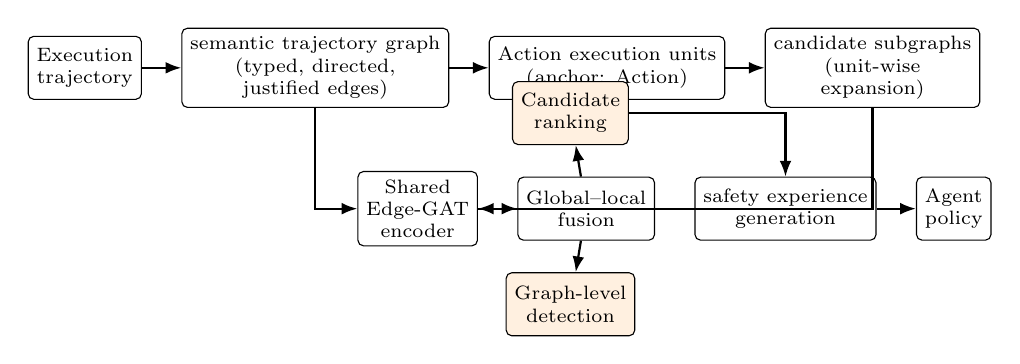
\begin{tikzpicture}[
  node distance=4mm and 5mm,
  box/.style={draw, rounded corners=2pt, align=center, font=\scriptsize, inner sep=3pt, minimum height=8mm},
  outbox/.style={box, fill=orange!12},
  arr/.style={-{Latex[length=2mm]}, thick},
  lab/.style={font=\tiny, align=center}
]
\node[box] (traj) {Execution\\trajectory};
\node[box, right=of traj] (graph) {\stg{}\\(typed, directed,\\justified edges)};
\node[box, right=of graph] (unit) {\aeu{}s\\(anchor: Action)};
\node[box, right=of unit] (cand) {\csg{}s\\(unit-wise\\expansion)};
\node[box, below=8mm of graph, xshift=13mm] (enc) {Shared\\Edge-GAT\\encoder};
\node[box, right=of enc] (fuse) {Global--local\\fusion};
\node[outbox, below=4mm of fuse, xshift=-2mm] (detect) {Graph-level\\detection};
\node[outbox, above=4mm of fuse, xshift=-2mm] (loc) {Candidate\\ranking};
\node[box, right=of fuse] (exp) {\sexp{}\\generation};
\node[box, right=of exp] (agent) {Agent\\policy};
\draw[arr] (traj) -- (graph);
\draw[arr] (graph) -- (unit);
\draw[arr] (unit) -- (cand);
\draw[arr] (cand) |- (enc);
\draw[arr] (graph) |- (enc);
\draw[arr] (enc) -- (fuse);
\draw[arr] (fuse) -- (detect);
\draw[arr] (fuse) -- (loc);
\draw[arr] (loc) -| (exp);
\draw[arr] (exp) -- (agent);
\end{tikzpicture}}
\caption{The overall architecture of the proposed framework. The upper part represents \stg{} construction and \aeu{}-anchored \csg{} extraction; the lower left part corresponds to shared edge-attention encoding and global--local fusion; and the right part illustrates graph-level detection, candidate ranking, and \sexp{} generation that conditions the agent policy.}
\label{fig:overview}
\end{figure}

\subsection{Notations}

We summarize the notation used throughout this section. Each execution trajectory $\mathcal{T}$ is represented as a directed attributed graph $G=(V,E,X_V,X_E)$ following Eq.~\eqref{eq:graph} in \S\ref{sec:problem}, where $V$ is the node set, $E\subseteq V\times V$ is the directed edge set following execution flow, $X_V$ collects node features, and $X_E$ collects edge features. Each node carries one of the four execution roles in Table~\ref{tab:nodetypes}, and each edge carries one of the five relation types in Table~\ref{tab:edgetypes} together with a direction and a justification text $t_{ij}$. For an action $a\in V$, its \aeu{} is denoted $U_a$ following Eq.~\eqref{eq:unit}, and the \csg{} set of the trajectory is $\mathcal{C}=\{C_1,\dots,C_K\}$ with $K$ candidates grown by Eqs.~\eqref{eq:cand0}--\eqref{eq:cand}. A detection model is represented as $f_\theta$, parameterized by $\theta$; given $G$ and $\mathcal{C}$, it outputs a graph-level score $p_G\in[0,1]$ and candidate scores $\{p_k\}$ with margins $\{m_k\}$. Training minimizes a composite objective $\mathcal{L}_{\mathrm{total}}(\theta)$ defined over graph labels $y_G$, paired normal/anomalous trajectories, and pseudo-labeled candidates. Unless otherwise specified, $d$ denotes the hidden dimension, $L$ the number of encoder layers, and $B$ the maximum candidate size measured in nodes.

\subsection{Chunk-Aware Node and Edge Representation}

In this subsection, we construct the node and edge features that feed the shared encoder. Node texts in trajectories range from a tool parameter to a multi-paragraph reflection, and a single pooled vector would blur exactly the spans that carry risk signals. Specifically, each node text is split into overlapping token chunks $\{c_{ij}\}$, encoded independently by a sentence encoder~\cite{reimers2019sentencebert,gao2021simcse}, and each chunk receives a risk gate:
\begin{equation}
z_{ij}=\operatorname{TextEncoder}(c_{ij}),\qquad
r_{ij}=\sigma(\operatorname{MLP}(z_{ij})),
\label{eq:riskgate}
\end{equation}
where $z_{ij}\in\mathbb{R}^{d}$ is the embedding of chunk $j$ of node $i$, and $r_{ij}\in(0,1)$ is the gate value that amplifies chunks whose content resembles risk-bearing language. The gated chunks are aggregated by max pooling into the node text representation:
\begin{equation}
h_i^{\mathrm{text}}=\max_j\!\left(\phi(z_{ij})\odot(1+r_{ij})\right),
\label{eq:chunkpool}
\end{equation}
where $\phi(\cdot)$ is a linear projection that aligns chunk embeddings with the node feature space and $\odot$ denotes element-wise multiplication; taking the maximum over gates keeps the most risk-salient chunk of each node. The final node feature concatenates $h_i^{\mathrm{text}}$ with a node-type embedding, a relative position encoding, and the text length. Every directed edge $(i,j)$ encodes its justification text, relation type, and direction:
\begin{equation}
g_{ij}=\operatorname{MLP}_E\!\big(\big[\operatorname{TextEncoder}(t_{ij});\,e_{\mathrm{rel}(i,j)};\,e_{\mathrm{dir}(i,j)}\big]\big),
\label{eq:edgefeat}
\end{equation}
where $t_{ij}$ is the justification text of \S\ref{sec:data}, $e_{\mathrm{rel}}$ and $e_{\mathrm{dir}}$ are learnable embeddings of the relation type in Table~\ref{tab:edgetypes} and the execution direction, and $[\cdot\,;\cdot]$ denotes concatenation. This design allows every inferred dependency to remain auditable, since its feature is grounded in the quotation that supports it. Encoder identity, chunk length, overlap, and dimensions are reported in \tbd{TBD-ENCODER-CONFIGURATION}.

\subsection{Action Execution Units and Candidate Subgraphs}

In this subsection, we construct the \aeu{}s and the \csg{}s from the graph built in \S\ref{sec:data}. For each action $a$, the unit $U_a$ in Eq.~\eqref{eq:unit} is recovered directly from the graph structure: the reasoning chain $R_a$ follows semantic in-edges backward from $a$; the inputs $I_a$ follow the same edges one step further or terminate at the triggering state; the output $O_a$ follows the \texttt{computes\_from} edge; and the reflections $F_a$ attach through \texttt{reflects} edges. Figure~\ref{fig:unit} illustrates a unit inside a running example with branches and a convergence. Unit dependencies are then built from state reuse: if the output state of $U_{a_i}$ is consumed by $U_{a_j}$, we add a unit dependency $U_{a_i}\rightarrow U_{a_j}$, and candidates grow from an anchor unit by adding complete predecessor units layer by layer, following Eqs.~\eqref{eq:cand0}--\eqref{eq:cand} under the six constraints of \S\ref{sec:problem}. Independent branches form separate candidates, so evidence from one branch is not diluted by another; converging actions may additionally form a joint-context candidate, so composition risks---where two individually innocuous operations jointly produce harm---are represented. The budget constraint guarantees that every action keeps at least one anchored candidate, so localization can never silently drop an operation. This construction ensures that every candidate is a complete, connected slice of an actual execution, which is the property that fixed-hop neighborhoods lack. Candidate coverage and size statistics are reported in \tbd{TBD-CANDIDATE-COVERAGE}.

\begin{figure}[t]
\centering
\resizebox{\linewidth}{!}{%
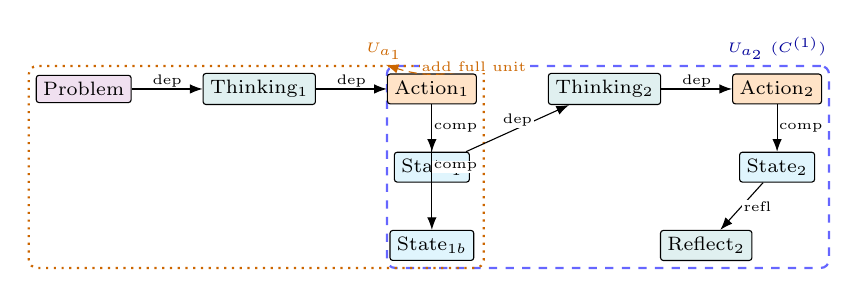
\begin{tikzpicture}[
  node distance=6mm and 9mm,
  pnode/.style={draw, rounded corners=1pt, fill=violet!12, font=\scriptsize, inner sep=2.5pt, minimum width=9mm},
  tnode/.style={draw, rounded corners=1pt, fill=teal!12, font=\scriptsize, inner sep=2.5pt, minimum width=9mm},
  anode/.style={draw, rounded corners=1pt, fill=orange!22, font=\scriptsize, inner sep=2.5pt, minimum width=9mm},
  snode/.style={draw, rounded corners=1pt, fill=cyan!12, font=\scriptsize, inner sep=2.5pt, minimum width=9mm},
  arr/.style={-{Latex[length=1.6mm]}, font=\tiny},
  el/.style={font=\tiny, fill=white, inner sep=0.5pt}
]
\node[pnode] (p) {Problem};
\node[tnode, right=of p] (t1) {Thinking$_1$};
\node[anode, right=of t1] (a1) {Action$_1$};
\node[snode, below=of a1] (s1) {State$_1$};
\node[tnode, right=of a1] (t2) {Thinking$_2$};
\node[anode, right=of t2] (a2) {Action$_2$};
\node[snode, below=of a2] (s2) {State$_2$};
\node[tnode, below=of s2, xshift=-9mm] (f2) {Reflect$_2$};
\node[snode, below=of s1] (s1b) {State$_{1b}$};
\draw[arr] (p) -- node[el, above] {dep} (t1);
\draw[arr] (t1) -- node[el, above] {dep} (a1);
\draw[arr] (a1) -- node[el, right] {comp} (s1);
\draw[arr] (a1) -- node[el, right] {comp} (s1b);
\draw[arr] (s1) -- node[el, above] {dep} (t2);
\draw[arr] (t2) -- node[el, above] {dep} (a2);
\draw[arr] (a2) -- node[el, right] {comp} (s2);
\draw[arr] (s2) -- node[el, right] {refl} (f2);
\begin{scope}[on background layer]
\node[draw=blue!60, thick, dashed, rounded corners=3pt, fit=(s1)(t2)(a2)(s2)(f2), inner sep=2.5pt] (u2) {};
\node[draw=orange!80!black, thick, dotted, rounded corners=3pt, fit=(p)(t1)(a1)(s1)(s1b), inner sep=2.5pt] (u1) {};
\end{scope}
\node[font=\tiny, blue!60!black, above=0.5mm of a2] {$U_{a_2}$ ($C^{(1)}$)};
\node[font=\tiny, orange!80!black, above=0.5mm of a1, xshift=-6mm] {$U_{a_1}$};
\draw[arr, orange!80!black, densely dashed] (u1.north east) to[bend left=18] node[el, above right=0mm and -2mm] {add full unit} (u2.north west);
\end{tikzpicture}}
\caption{The construction of \aeu{}s and unit-wise \csg{}s. The boxed regions mark complete units: the anchored unit $U_{a_2}$ contains the full input state, reasoning chain, action, output state, and reflection, and candidate growth adds complete predecessor units ($U_{a_1}$), never partial hops. Branch outputs of $a_1$ stay inside their own units and feed separate candidates.}
\label{fig:unit}
\end{figure}

\subsection{Shared Edge-Attention Encoding and Contextual Scoring}

In this subsection, we encode the full trajectory and all candidates with one shared encoder and score candidates in context. Full trajectories and \csg{}s must be comparable in a single representation space; otherwise the contextual comparison below degenerates. Specifically, a directed edge-attention layer aggregates from true in-edge neighbors only, with attention determined jointly by source, target, and edge representations:
\begin{equation}
h_i^{(l+1)}=\operatorname{ResNorm}\!\left(
h_i^{(l)}+
\sum_{j:(j,i)\in E}
\alpha_{ji}^{(l)}\operatorname{Msg}(h_j^{(l)},g_{ji})
\right),
\label{eq:edgegat}
\end{equation}
where $h_i^{(l)}$ is the state of node $i$ at layer $l$, $g_{ji}$ is the edge feature of Eq.~\eqref{eq:edgefeat}, $\alpha_{ji}^{(l)}$ is the attention coefficient computed from the pair of node states and the edge representation, $\operatorname{Msg}(\cdot)$ is the message function, and $\operatorname{ResNorm}(\cdot)$ is a residual-and-normalization block that stabilizes depth. Because edge features enter both the attention logits and the message, justification text and relation type directly modulate information flow, the property that relational and heterogeneous encoders establish as necessary for typed graphs~\cite{schlichtkrull2017modeling,hu2020heterogeneous}. Graph-level representations pool node states:
\begin{equation}
h_G=\operatorname{MeanPool}(\{h_i\})\,\Vert\,\operatorname{MaxPool}(\{h_i\}),
\label{eq:pool}
\end{equation}
where $\Vert$ denotes concatenation; Eq.~\eqref{eq:pool} is computed identically for the full graph $G$ and each \csg{} $C_k$, and both pass through a shared LayerNorm so that their scales are aligned.

For finer granularity, each candidate is scored \emph{in context}: the same operation can be legitimate in one trajectory and fatal in another, so the candidate representation is compared against the full-graph representation through similarity, difference, and product terms:
\begin{equation}
q_k=\big[h_{C_k};\,h_G;\,|h_{C_k}-h_G|;\,h_{C_k}\odot h_G\big],
\label{eq:qk}
\end{equation}
from which a candidate margin and probability are read:
\begin{equation}
m_k=f_\theta(q_k),\qquad p_k=\sigma(m_k),
\label{eq:mk}
\end{equation}
where $f_\theta$ is a scoring head parameterized by $\theta$, $m_k$ is the candidate margin, and $p_k$ is the probability that candidate $C_k$ is a risk locus. The local branch fuses the strongest candidate with the average of the top-ranked candidates, so evidence scattered over several operations is not lost:
\begin{equation}
S_{\mathrm{local}}=\alpha\max_k m_k+(1-\alpha)\operatorname{Mean}(\operatorname{TopK}(\{m_k\})),
\label{eq:slocal}
\end{equation}
and the final graph-level score blends the full-graph and local branches:
\begin{equation}
S_G=\beta S_{\mathrm{full}}+(1-\beta)S_{\mathrm{local}},\qquad p_G=\sigma(S_G),
\label{eq:sg}
\end{equation}
where $S_{\mathrm{full}}$ is the score read from $h_G$ by the same head, and $\alpha,\beta\in(0,1)$ are sigmoid-parameterized and learned from data rather than fixed, letting the training distribution decide how much localization contributes to detection. This design allows the local branch to contribute operation-level evidence that a whole-graph score cannot express, while the global branch supplies behavioral context that a subgraph alone lacks.

\subsection{Weakly Supervised Optimization}

In this subsection, we train the detector and the ranker jointly without action-level annotations. Complete action-level labels are scarce, while graph labels are abundant and paired normal/anomalous runs of the same task exist by construction of the corpora. Specifically, the total loss combines four terms:
\begin{equation}
\mathcal{L}_{\mathrm{total}}
=\mathcal{L}_{\mathrm{graph}}
+\lambda_p\mathcal{L}_{\mathrm{pseudo}}
+\mathcal{U}(\mathcal{L}_{\mathrm{normal}};s_n)
+\mathcal{U}(\mathcal{L}_{\mathrm{rank}};s_r),
\label{eq:ltotal}
\end{equation}
where $\mathcal{L}_{\mathrm{graph}}$ is the graph-level cross-entropy on $y_G$; $\mathcal{L}_{\mathrm{pseudo}}$ builds candidate pseudo-labels from paired trajectories, marking the candidates anchored at actions that changed between the anomalous and the normal run of the same task as positive within their anomalous graph; $\mathcal{L}_{\mathrm{normal}}$ suppresses high candidate scores inside normal graphs, discouraging a trivial solution in which every candidate is suspicious; and $\mathcal{L}_{\mathrm{rank}}$ requires that, for a task with one normal and one anomalous run, the anomalous graph's local score exceeds the normal graph's. Because the three auxiliary terms have different noise levels, they are combined through bounded uncertainty weighting in the spirit of multi-task loss balancing~\cite{kendall2017multitask}:
\begin{equation}
v=\operatorname{softplus}(s),\qquad w=\exp(-v)\in(0,1],
\label{eq:uw}
\end{equation}
\begin{equation}
\mathcal{U}(\mathcal{L};s)=w\,\mathcal{L}+v,
\label{eq:uw2}
\end{equation}
where $s$ is the learnable uncertainty parameter of the corresponding auxiliary term. The bound keeps weights in $(0,1]$, so a noisy auxiliary term is down-weighted but never dominates by inflating its own uncertainty.

\subsection{Safety Experience Generation}
\label{sec:method-exp}

In this subsection, we convert the localized evidence into knowledge that changes agent behavior. Detection without a locus cannot be acted upon, and a locus without transferable knowledge is lost at the end of the run. Specifically, at inference, a threshold $\tau$ tuned on validation data gates the graph-level decision, and only flagged trajectories undergo candidate ranking. Among near-tied candidates the smaller candidate is preferred, and heavily overlapping candidates are deduplicated; the Top-1 candidate serves as the primary risk evidence and the remaining top-ranked candidates serve as auxiliary evidence for evaluation. The \sexp{} generator receives only the detection scores, the anchor action, local node texts, the true semantic edges, and their justifications---\emph{never} the ground-truth label---and emits a structured record:
\begin{center}
\small
\texttt{risk\_type}, \texttt{what\_went\_wrong}, \texttt{warning\_signals}, \texttt{recommended\_agent\_policy}, \texttt{supporting\_node\_ids}, \texttt{confidence}.
\end{center}
The record is grounded by construction: \texttt{supporting\_node\_ids} points into the candidate, so every claim can be checked against nodes and edges of the original graph. The experience is consumed as \emph{soft safety context}, not as a hard block: before subsequent tool calls, the agent re-checks goal consistency, input trustworthiness, parameter and data-scope authorization, and potential disclosure or unauthorized consequence of the pending operation. This design separates the contribution of the detector (when to act) from that of the localized evidence (what to check), which the controlled conditions of \S\ref{sec:defense} isolate experimentally. Qualitative cases are reported in \tbd{TBD-QUALITATIVE-CASES}.

\subsection{Complexity Analysis}

The computational complexity of the framework can be broken down by stage, each contributing differently based on the operations involved. Graph construction and candidate extraction are linear passes over the trajectory: recovering units and growing candidates visit each node and edge a constant number of times, giving $O(|V|+|E|)$ per trajectory. Text encoding dominates preprocessing: with $n_c$ chunks per node on average and a transformer encoder whose self-attention costs $O(n_t^2)$ for a chunk of $n_t$ tokens, encoding all nodes costs $O(|V|\,n_c\,n_t^{2})$, and encoding edge justifications adds $O(|E|\,n_t^{2})$. The shared Edge-GAT costs $O(L(|E|d+|V|d^{2}))$ per forward pass on the full graph; since each candidate contains at most $B$ nodes and $B$ edges, encoding all $K$ candidates adds $O(K\,L\,(Bd+Bd^{2}))$, and contextual scoring adds $O(Kd)$ for the fusion heads. Experience generation is a single generation call over the Top-1 candidate, whose prompt is bounded by $B$ nodes, so its cost is independent of the trajectory length. In summary, the training complexity is
$O(|V|n_cn_t^{2}+|E|n_t^{2}+L(|E|d+|V|d^{2})+KL(Bd+Bd^{2}))$,
and inference adds only one candidate-ranking pass over flagged trajectories. For a fixed candidate budget $K\cdot B$, the framework exhibits linear growth in trajectory size, in the same range as standard GNN encoders, which supports auditing long executions.

\begin{algorithm}[htbp]
\caption{Training, Inference, and Deployment Procedure of the Proposed Framework}
\label{alg:framework}
\begin{algorithmic}[1]
\Require trajectory corpus with graph labels $\{(\mathcal{T}_i,y_{G,i})\}$; paired normal/anomalous executions $\mathcal{P}$; validation-tuned threshold $\tau$; hyper-parameters.
\Ensure graph-level scores $\{p_G\}$; ranked candidates $\{p_k\}$; \sexp{} store $\mathcal{M}$.
\State \textit{/* Stage 1: graph construction and candidate extraction (offline, \S\ref{sec:data}) */}
\For{each trajectory $\mathcal{T}$}
  \State build the \stg{} $G$: Phase~1 fixes the execution skeleton, Phase~2 adds cross-step dependencies with justification texts $t_{ij}$ (\S\ref{sec:data});
  \State recover \aeu{}s by Eq.~\eqref{eq:unit} and grow \csg{}s by Eqs.~\eqref{eq:cand0}--\eqref{eq:cand} under the six constraints of \S\ref{sec:problem};
\EndFor
\State \textit{/* Stage 2: representation, encoding, and weakly supervised optimization */}
\For{each training epoch}
  \For{each mini-batch of graphs and candidate sets $(G,\mathcal{C})$}
    \State encode chunk-gated node features and edge features by Eqs.~\eqref{eq:riskgate}--\eqref{eq:edgefeat};
    \State encode $G$ and all candidates with the shared Edge-GAT by Eqs.~\eqref{eq:edgegat}--\eqref{eq:pool};
    \State compute candidate margins and graph-level scores by Eqs.~\eqref{eq:qk}--\eqref{eq:sg};
    \State build paired pseudo-labels from $\mathcal{P}$; optimize $\mathcal{L}_{\mathrm{total}}$ in Eq.~\eqref{eq:ltotal} with bounded weights in Eqs.~\eqref{eq:uw}--\eqref{eq:uw2};
  \EndFor
\EndFor
\State \textit{/* Stage 3: inference and experience generation */}
\For{each run with $p_G\geq\tau$}
  \State rank candidates by $p_k$; deduplicate overlapping candidates and prefer the smaller near-tied one;
  \State generate the \sexp{} from the Top-1 candidate: risk type, failure description, warning signals, recommended policy, supporting node ids, and confidence (\S\ref{sec:method-exp});
  \State append the experience to the store $\mathcal{M}$;
\EndFor
\State \textit{/* Stage 4: deployment loop with experience-conditioned execution */}
\While{the agent executes a new task}
  \State before each tool call, apply the soft-context re-checks induced by $\mathcal{M}$: goal consistency, input trustworthiness, parameter and data-scope authorization, and disclosure risk (\S\ref{sec:method-exp});
  \State execute the tool call and extend the \stg{} with the observed records;
  \If{the run is flagged ($p_G\geq\tau$)}
    \State compile the localized evidence into a new \sexp{} and append it to $\mathcal{M}$;
  \EndIf
\EndWhile
\State \Return graph-level decisions, ranked candidates, and the \sexp{} store $\mathcal{M}$.
\end{algorithmic}
\end{algorithm}

\section{Experimental Setup and Evaluation Design}
\label{sec:experiments}

\subsection{Protocol}
All experiments follow one protocol across corpora and tasks. Data are split under \tbd{TBD-SPLIT-PROTOCOL}, with grouping that prevents the same task family, site, or injected payload family from spanning training and test splits, and leakage controls audited as specified in \tbd{TBD-DATA-LEAKAGE-CONTROL}. Stochastic stages are repeated over \tbd{TBD-RANDOM-SEEDS} seeds. The anomaly class is expected to be the minority in every corpus; therefore \emph{PR-AUC} and anomaly-class \emph{precision/recall/F1} are treated as the primary detection statistics, with accuracy reported only as a reference point, since accuracy can be dominated by the majority class under imbalance. Sensitivity of operating points is analyzed separately from ranking quality in \tbd{TBD-THRESHOLD-ANALYSIS}.

\subsection{Baselines and Input Paradigms}
\label{sec:baselines}
Baselines cover six families, spanning the input paradigms that matter for interpretation (Table~\ref{tab:main}). (i)~\emph{Text-trajectory screening}: safety models and classifiers that read the trajectory as flat text or segmented text, representative of guard-model practice~\cite{inan2023llama,liu2024calibration}. (ii)~\emph{Generic graph neural networks}: message passing without relation or edge awareness~\cite{velikovi2017graph}. (iii)~\emph{Relation- and edge-aware graph models}: encoders that consume typed, directed, attributed graphs~\cite{schlichtkrull2017modeling,hu2020heterogeneous,brody2021attentive}. (iv)~\emph{Graph anomaly detection}: graph-level scoring methods~\cite{tang2022rethinking,liu2021anomaly,wang2026glass}. (v)~\emph{LLM-as-a-Judge}: generative judges over whole trajectories~\cite{zheng2023judging,yuan2024rjudge,zhuge2024agentasajudge}. (vi)~\emph{Content-safety guard models}: deployed moderation systems applied to serialized runs. The final baseline roster, configurations, and the fairness protocol are recorded in \tbd{TBD-BASELINE-LIST} and \tbd{TBD-BASELINE-CONFIGURATIONS}. One reporting rule is fixed in advance: methods that read flat text and methods that read the \stg{} are \emph{not} presented as operating under identical input conditions, and comparison tables group them accordingly (\tbd{TBD-FAIR-COMPARISON-PROTOCOL}).

\begin{table}[t]
\caption{Main graph-level detection comparison. Groups are separated by input paradigm; cells are completed from the experiments.}
\label{tab:main}
\resizebox{\linewidth}{!}{%
\begin{tabular}{lccccc}
\toprule
Method & ROC-AUC & PR-AUC & $F_1^{anom}$ & FPR & Bal-Acc \\
\midrule
\emph{Text-trajectory screening} & & & & & \\
\emph{Generic GNN} & & & & & \\
\emph{Relation/edge-aware GNN} & & & & & \\
\emph{Graph anomaly detection} & & & & & \\
\emph{LLM-as-a-Judge} & & & & & \\
\emph{Guard model} & & & & & \\
\emph{Ours (full)} & & & & & \\
\midrule
\multicolumn{6}{c}{\tbd{TBD-MAIN-DETECTION-TABLE}} \\
\bottomrule
\end{tabular}}
\end{table}

\subsection{Detection Questions}
\textbf{RQ1.} Does joint global--local modeling improve graph-level detection over single-granularity scoring? The full model is compared against full-graph-only and Action-subgraph-only variants under the global/local ablation \tbd{TBD-GLOBAL-LOCAL-ABLATION}; the outcome, its significance, and the threshold analysis are recorded in \tbd{TBD-DETECTION-SIGNIFICANCE} and \tbd{TBD-THRESHOLD-ANALYSIS}. The mechanism claim under test is that the local branch adds operation-level evidence that a whole-graph score cannot express, while the global branch supplies behavioral context that a subgraph alone lacks; the ablation is designed so that each branch's marginal value is directly readable from the table.

\subsection{Localization Questions}
\textbf{RQ2.} Does localization recover the responsible operations? Metrics are Action Hit@1, Hit@$K$/Recall@$K$, node- and edge-level IoU between the predicted candidate and the ground-truth changed-action context, and candidate size. Candidate-generation coverage is reported separately in \tbd{TBD-CANDIDATE-COVERAGE} and never substituted for final localization: a candidate set that contains the true locus does not imply the model ranks it first. Results appear in \tbd{TBD-LOCALIZATION-RESULTS}; qualitative cases are curated in \tbd{TBD-QUALITATIVE-CASES}.

\begin{table}[t]
\caption{Action-level localization. Coverage of the candidate stage is reported separately from final ranking.}
\label{tab:loc}
\resizebox{\linewidth}{!}{%
\begin{tabular}{lccccc}
\toprule
Candidate scheme & Hit@1 & Hit@$K$ & IoU$_n$ & IoU$_e$ & Size \\
\midrule
\emph{Fixed-hop candidates} & & & & & \\
\emph{Action-unit candidates (ours)} & & & & & \\
\midrule
\multicolumn{6}{c}{\tbd{TBD-LOCALIZATION-TABLE}} \\
\bottomrule
\end{tabular}}
\end{table}

\textbf{RQ3.} Is the \aeu{} the right atomic unit? The central comparison is fixed-hop candidate construction versus unit-wise construction, holding the encoder and objective fixed, on coverage, final Hit@$K$, IoU, and candidate size (\tbd{TBD-FIXED-HOP-VS-ACTION-UNIT}). This isolates the representation choice from the scoring machinery: any difference must come from where candidate boundaries fall, not from parameters.

\subsection{Ablation Questions}
\textbf{RQ4.} Which representation and objective components carry the effect? The planned grid removes: edge justification text; relation type; directionality; replaces chunk-risk-max pooling with truncation or chunk-mean; fixes versus learns $\alpha,\beta$; removes the shared LayerNorm alignment; removes paired pseudo-labels; and replaces bounded uncertainty weighting with fixed auxiliary weights. Results are recorded in \tbd{TBD-REPRESENTATION-ABLATIONS} and \tbd{TBD-OBJECTIVE-ABLATIONS} (Table~\ref{tab:ablation}).

\begin{table}[t]
\caption{Representation and objective ablations.}
\label{tab:ablation}
\begin{tabular}{lccc}
\toprule
Variant & ROC-AUC & PR-AUC & Hit@1 \\
\midrule
\emph{Representation ablations} & & & \\
\emph{Objective ablations} & & & \\
\midrule
\multicolumn{4}{c}{\tbd{TBD-ABLATION-TABLE}} \\
\bottomrule
\end{tabular}
\end{table}

\textbf{RQ5.} Does the pipeline transfer across input paradigms and corpora? The same protocol is run on \tbd{TBD-DATASET-NAME-A}, \tbd{TBD-DATASET-NAME-B}, and \tbd{TBD-PRIVATE-DATASET-NAME} with per-corpus statistics in \tbd{TBD-DATASET-STATISTICS}; cross-corpus variation is where representation choices are most likely to matter, since browsing-style runs and tool-benchmark runs differ in graph shape.

\section{Experience-Based Defense Evaluation}
\label{sec:defense}

\subsection{Closed-Loop Protocol}
The defense experiment measures whether localized evidence changes agent behavior on future, similar situations, and---critically---which part of the pipeline produces the change. The protocol instantiates the agent under the target attack suite, injects \sexp{}s as \emph{soft safety context} before each tool call, and compares attack success and normal utility across conditions. All conditions share the agent configuration, the tool inventory, and the task distribution; the \emph{only} manipulated variable is the content of the safety context. Attack success rate and task success rate follow the definitions of the underlying benchmarks~\cite{debenedetti2024agentdojo,zhan2024injecagent,tur2025safearena,levy2024stwebagentbench}, and we additionally track \emph{false triggers} (defensive interventions on benign operations) and intervention cost. Statistical comparisons between paired conditions use \tbd{TBD-DEFENSE-SIGNIFICANCE}. Because adversaries adapt~\cite{zhan2025adaptive,syros2026muzzle}, reported suppression reflects the studied attack suite rather than a permanent property, which the deployment discussion in \S\ref{sec:vision} takes up. The full defense table and its results are recorded in \tbd{TBD-DEFENSE-TABLE} (Table~\ref{tab:defense}).

\begin{table}[t]
\caption{Defense conditions and outcomes. Conditions differ only in the safety-context content; numbers are completed from the experiments.}
\label{tab:defense}
\resizebox{\linewidth}{!}{%
\begin{tabular}{lccccc}
\toprule
Condition & ASR$\downarrow$ & Task SR & False trig. & Cost & $\Delta$ASR \\
\midrule
Attack-only baseline & & & & -- & -- \\
Generic warning & & & & & \\
Full-graph experience & & & & & \\
Random subgraph experience & & & & & \\
Detected Action-subgraph exp. (ours) & & & & & \\
Oracle Action-subgraph exp. & & & & & \\
\midrule
\multicolumn{6}{c}{\tbd{TBD-DEFENSE-TABLE}} \\
\bottomrule
\end{tabular}}
\end{table}

\subsection{Controlled Conditions}
\label{sec:defense-conditions}
Six conditions separate confounds that generic warnings cannot. \emph{Attack-only} calibrates the undefended success rate. \emph{Generic warning} injects a fixed alert that an attack may be present, with no localized evidence; it captures placebo effects of ``be careful'' prompting and is the condition most defenses implicitly implement. \emph{Full-graph experience} injects the generator's output over the \emph{entire} trajectory, testing whether the benefit comes from localization or merely from more grounded text. \emph{Random subgraph experience} injects an experience grounded in a random connected \csg{}, controlling for grounding structure without risk relevance. \emph{Detected Action-subgraph experience} is the full pipeline: the detector flags the run, the ranker selects the candidate, and the generator compiles the experience. \emph{Oracle Action-subgraph experience} grounds the experience in the true risk locus, bounding what perfect localization could achieve. The gap between the detected and oracle conditions is therefore an upper-bound estimate of the localization component's headroom, and the gap between detected and generic conditions isolates the value of operation-level evidence over generic caution.

\subsection{What Each Comparison Answers}
Three contrasts carry the interpretation. Detected versus \emph{generic} answers whether structured, operation-anchored evidence matters beyond alerting the agent that something might be wrong. Detected versus \emph{full-graph} answers whether localization, rather than additional grounded context, is the operative ingredient. Detected versus \emph{random subgraph} answers whether the grounding subgraph must be risk-relevant, not merely well-formed and connected. Utility is evaluated on normal runs, where a well-calibrated system must not intervene: false-trigger rate and utility degradation on the normal set are reported alongside attack suppression, since a defense that refuses benign operations fails the deployment test regardless of its attack success reduction. Cross-configuration generalization---experiences generated from one agent configuration consumed by another---is reported in \tbd{TBD-DEFENSE-TABLE} as an explicit column, because \sexp{}s are intended as reusable artifacts rather than session-bound outputs. Qualitative examples of generated experiences and induced policy changes appear in \tbd{TBD-QUALITATIVE-CASES}.

\section{Implications for the Agentic Web}
\label{sec:vision}

The Brave New Ideas track asks what the Web could become if a capability existed that does not exist today. We argue that action-centered execution auditing is that kind of capability, and we sketch what changes if it works at Web scale.

\paragraph{From content auditing to execution auditing.}
The Web's existing safety infrastructure---spam filters, content moderation, phishing detection, provenance signals---inspects \emph{content} at fetch time. For agents, the dangerous event is not the fetched byte but the executed operation, and attacks can be invisible in content and outcome alike~\cite{lee2026will}. If browsers, agent runtimes, and tool protocols emit trajectory graphs as a first-class artifact---the same way access logs and network traces are emitted today---then every agent-mediated action carries an auditable record of what state motivated it, what reasoning justified it, and what it changed. Detection and localization over such records generalize beyond prompt injection: any policy violation, error, or fraud that manifests in execution structure becomes addressable with the same substrate, including failures that outcome-based evaluation misses~\cite{mohammadi2026trajectoryjudge,deng2026defa}. This is a concrete, engineering-shaped path from today's ad-hoc guardrails toward execution-layer trust for the agentic Web~\cite{yang2025agentic,ng2026agent}.

\paragraph{Experiences as a portable safety layer.}
The \sexp{} format is deliberately an artifact, not a log line: it is small, structured, grounded in cited node identifiers, and written for a consumer agent rather than a human analyst. If experiences accumulate across runs, sites, and agent configurations, safety knowledge stops being bound to a single deployment---the failure a search agent suffers today can protect a booking agent tomorrow, and the memory-and-skill externalization trend of the field~\cite{zhou2026externalization,zhao2023expel,allard2026experiential} extends from competence to safety. The defense conditions of \S\ref{sec:defense} are designed to measure exactly the property this vision needs: whether an experience grounded in localized evidence transfers beyond the session that produced it.

\paragraph{Open problems the substrate raises.}
An execution-audit layer creates problems we do not solve here. \emph{Standardization}: trajectory-graph emission needs schema-level agreement among runtimes, in the spirit of emerging tool-protocol standards~\cite{hou2025model,zhang2025security}. \emph{Privacy}: graphs record how agents act on behalf of users, so emission policies must decide what is stored, for how long, and under whose access control. \emph{Experience pollution}: shared experience pools can be poisoned, and an attacker who understands the format can craft content that generates misleading experiences; provenance and robustness of the experience channel are prerequisites for the ecosystem, echoing lessons from repository- and knowledge-poisoning research. \emph{Governance}: if audits attribute actions to specific agent configurations, the substrate becomes evidence in accountability disputes, which is a feature for site operators and a liability question for agent vendors. We state these as open problems because they require the community-level agreement that a research paper cannot produce; what this paper contributes is the demonstration that the substrate's core operation---joint detection, operation-level localization, and grounded experience generation---is learnable at all.

\section{Conclusion}
We reformulated the safety of tool-using Web agents as joint graph-level detection and operation-level localization over execution-grounded \stg{}s, anchored risk at complete \aeu{}s instead of fixed-hop neighborhoods, learned both tasks jointly through a \csmil{} model with shared edge-attention encoding, graph labels, and paired weak supervision, and closed the loop by compiling localized evidence into structured \sexp{}s that condition future agent behavior. The controlled defense design separates the effect of localized evidence from generic alerting, and the formulation gives the emerging agentic Web a substrate---trajectory graphs as first-class artifacts---on which execution auditing, cross-agent experience sharing, and governance can build. The approach's power is bounded by graph-construction coverage and by the faithfulness of paired weak supervision, and establishing robustness to adaptive adversaries and experience pollution remains future work; what this paper establishes is that detection, localization, and defense over execution structure is a coherent, learnable, and Web-relevant research direction.

\bibliographystyle{ACM-Reference-Format}
\bibliography{refs}

\end{document}